%%%%%%%%%%%%%%%%%%%%%%% file typeinst.tex %%%%%%%%%%%%%%%%%%%%%%%%%
%
% This is the LaTeX source for the instructions to authors using
% the LaTeX document class 'llncs.cls' for contributions to
% the Lecture Notes in Computer Sciences series.
% http://www.springer.com/lncs       Springer Heidelberg 2006/05/04
%
% It may be used as a template for your own input - copy it
% to a new file with a new name and use it as the basis
% for your article.
%
% NB: the document class 'llncs' has its own and detailed documentation, see
% ftp://ftp.springer.de/data/pubftp/pub/tex/latex/llncs/latex2e/llncsdoc.pdf
%
%%%%%%%%%%%%%%%%%%%%%%%%%%%%%%%%%%%%%%%%%%%%%%%%%%%%%%%%%%%%%%%%%%%


\documentclass[runningheads,a4paper,12pt]{llncs}

\usepackage{amssymb}
\setcounter{tocdepth}{3}
\usepackage{graphicx}

\usepackage[utf8]{inputenc}

\usepackage{url}

\begin{document}

\mainmatter  % start of an individual contribution

% first the title is needed
\title{Resolução de Crazy Pavement:\\Utilização de restrições em Prolog}

% a short form should be given in case it is too long for the running head
%\titlerunning{Lecture Notes in Computer Science: Authors' Instructions}

% the name(s) of the author(s) follow(s) next
%
% NB: Chinese authors should write their first names(s) in front of
% their surnames. This ensures that the names appear correctly in
% the running heads and the author index.
%
\author{Nuno Martins and Gonçalo Ribeiro}
\authorrunning{FEUP: Programação em lógica}
% (feature abused for this document to repeat the title also on left hand pages)

% the affiliations are given next; don't give your e-mail address
% unless you accept that it will be published
\institute{Faculdade de Engenharias da Universidade do Porto}
%
% NB: a more complex sample for affiliations and the mapping to the
% corresponding authors can be found in the file "llncs.dem"
% (search for the string "\mainmatter" where a contribution starts).
% "llncs.dem" accompanies the document class "llncs.cls".
%

\toctitle{Lecture Notes in Computer Science}
\tocauthor{Authors' Instructions}
\maketitle


\begin{abstract}
O objetivo deste artigo é demonstrar a forma de como foi resolvido o problema de resolver o puzzle Crazy Pavement com o uso de restrições, no âmbito da unidade curricular de Programação em Lógica, do 3º ano do Mestrado Integrado em Engenharia Informática e Computação, na FEUP.
\keywords{Prolog Crazy Pavement Puzzle PLR Restrictions Solver}
\end{abstract}

\section{Introdução}

No âmbito da unidade curricular de Programação em Lógica, foi-nos proposto para o segundo trabalho prático a elaboração de um puzzle em Prolog, recorrendo ao uso de restrições lógicas.

O objetivo deste trabalho foi pôr em prática os conhecimentos adquiridos sobre programação em lógica com restrições. Uma restrição lógica é uma limitação ao domínio de uma variàvel lógica. A linguagem Prolog pertence à classe de linguagens CLP - Contraint Logic Programming. Esta classe de linguagens combina a declaratividade da programação em lógica com a eficiência da resolução de restrições, substituindo o método de pesquisa predefinido da programação em lógica - "generate and test" - por "constrain and generate".

A problemática central do nosso trabalho reside na tradução das regras de um puzzle em restrições lógicas. Isto passa pela escolha de uma estrutura viável para a representação de soluções, e adaptar as regras linguísticas do puzzle em restrições do domínio lógico desta estrutura.

\section{Descrição do problema}

Crazy pavement é um puzzle realizado num tabuleiro quadriculado, com largura e comprimento iguais, dividido em várias regiões.

O objetivo do puzzle consiste em sombrear estas regiões de forma a cumprir restrições arbitrárias, impostas sobre o número de células sombreadas por linha ou por coluna. 
Foram empregues restrições lógicas ao nível do código. O resultado final é um gerador de soluções funcional, com interface de texto.
 
\begin{figure} 
\centering
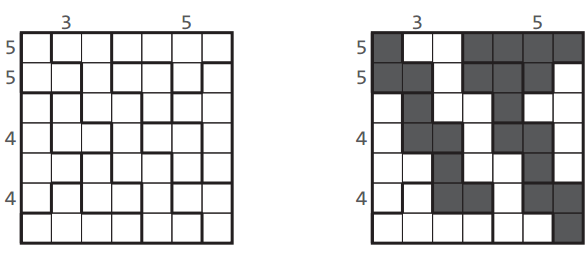
\includegraphics[height=3.2cm]{exemplo1.png}
\caption{Exemplo de um puzzle com as suas restrições e a respetiva solução} 
\label{fig:crazypavementexandsol}
\end{figure}

\newpage

\section{Abordagem}

Para representar o tabuleiro do jogo, foi usada uma estrutura genérica para representação de tabuleiros, que consiste numa lista de lista de elementos, em que cada elemento é um número positivo.Cada um destes números representa uma região, tendo as mesmas regiões índices iguais.

As restrições no numero de casas sombreadas são guardadas numa lista sob a forma [Linha1,N1,Linha2,N2,...], em que Linha refere ao índice da linha à qual vai ser aplicada a restrição, e N o número de casas sombreadas nessa linha.O mesmo conceito se aplica às colunas.

\begin{figure}
\centering
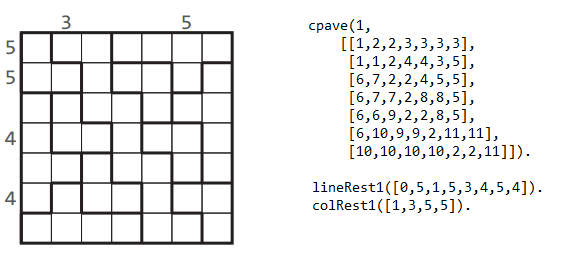
\includegraphics[height=3.2cm]{exemplo2.png}
\caption{Exemplo de um puzzle e a sua representação, assim como as suas restrições} 
\label{fig:crazypavementexandsol}
\end{figure}

\subsection{Variáveis de decisão}

As variáveis de decisão usadas para a resolução do problema estão presentes numa lista cujo comprimento é igual ao número de regiões existentes no puzzle.Este comprimento é encontrado através do predicado \textit{getBiggestN(+Board,-N)}, que retorna a casa com maior índice no tabuleiro.

Cada elemento desta lista pode tomar os valores 0 ou 1, indicando se a região com o mesmo índice está sombreada ou não.
\begin{figure}
\centering
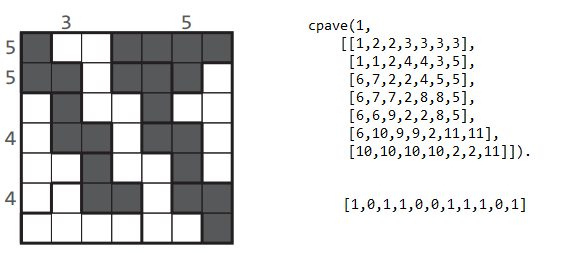
\includegraphics[height=3.2cm]{exemplo3.png}
\caption{Exemplo de um puzzle resolvido e a sua representação, e a sua solução} 
\label{fig:crazypavementexandsol}
\end{figure}

\newpage

\subsection{Restrições}

Existem 2 restrições impostas no problema.Estas são o número de casas sombreadas por cada linha e o número de casas sombreadas por cada coluna.

Estas são impostas pelos predicados \textit{allLinesMet(+Lines,+Board,-Solution)} e \textit{allColsMet(+Cols,+Board,-Solution)} , em que \textit{Board} é o tabuleiro, \textit{Lines/Cols} as restrições a ser impostas e \textit{Solution} a lista com as zonas a sombrear.

O funcionamento destes predicados consiste em iterar todos os elementos de uma linha/coluna, sendo um dos parametros de uma das funções auxiliares o número de casas nessa linha/coluna que deve ser sombreada.
Cada vez que é passada uma casa cujo índice na lista de solução esteja a 1, este contador é decrementado, sendo apenas este predicado verdadeiro se o contador estiver a 0 quando chegar ao fim da linha/coluna.


\section{Visualização da Solução}

Para iniciar a aplicação, deve ser consultado o ficheiro 'crazypave.pl' e corrido o predicado \textit{crazypave} .
Depois de executar o este predicado, serão pedidos ao utilizador as restrições a usar para as linhas, e quando todas colocadas, inserir '-1' para poder inserir as restrições de colunas.
Depois de inseridas estas , inserir '-1' novamente para encontrar a solução.
Alternativamente, pode-se correr os predicados \textit{test1,test2,test3,test4} para encontrar a solução de boards e respetivas restrições já predefinidas, sendo o 1º o puzzle fornecido no Moodle.

A forma que solução é demonstrada pode ser visualizada na figura abaixo, onde pode ser observado o tempo necessário a encontrar a solução, estatisticas e o tabuleiro no modo texto.



\begin{figure}
\centering
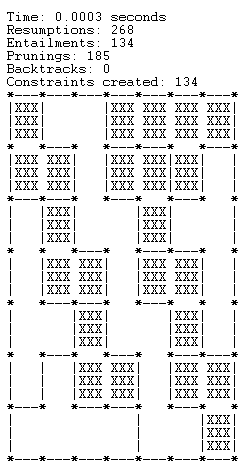
\includegraphics[height=6.5cm,width=4.5cm]{exemplo4.png}
\caption{Demonstração do resultado de correr o predicado test1} 
\label{fig:crazypavementexandsol}
\end{figure}

\section{Resultados}

Foram testados no total 4 puzzles, 1 com tamanho 7x7 e 3 com tamanho 10x10, tendo o ultimo um número superior de restrições.

Os resultados que foram obtidos não são conclusivos devido tanto ao pequeno número de puzzles encontrados na internet como à pequena dimensão destes.

No entanto, concluiu-se que:

\begin{itemize}
  \item Quantas mais restrições impostas, mais retrocessos ocorrem;
  \item Quantas mais regiões, mais retrocessos ocorrem;
  \item O tamanho do puzzle não tem influência no número de retrocessos;
\end{itemize}

Quanto ao tempo gasto, não podem ser tiradas conclusões, pois não foi encontrado nenhum puzzle que demorasse mais de 0.0001s a ser resolvido.



\section{Conclusão}

Como considerações finais, estamos satisfeitos com o trabalho que realizámos e concordamos que foi uma experiência enriquecedora e que de certa forma colocou à prova os nossos conhecimentos de lógica.

De momento, todos os puzzles são hardcoded. Reconhecemos que a implementação de uma funcionalidade que permitisse ao utilizador ler puzzles a partir de ficheiros sería uma melhoria conveniente, assim como a adição de um menu "how to play" para orientar novos utilizadores ao funcionamento do programa.

Visto que o cerne do nosso código - o predicado que gera soluções do puzzle - foi desenvolvido numa única aula prática, reconhecemos o poder da programação com restrições lógicas na resolução deste tipo de problemas combinatórios. É de nossa opinião que a mesma implementação num paradigma de linguagem imperativo (C, Java, etc.) resultaria num tempo desenvolvimento maior e num código mais extenso e complexo.

\end{document}
